\def\template{../template/}
\makeatletter \ifx\input@path\@undefined \def\input@path{{\template}} \else \g@addto@macro\input@path{{\template}} \fi \makeatother


% -- Documentclass --------------------------------------------------------%
\documentclass[pagenumoff]{kit-document}
\usepackage{CAMMP-settings}


% -- Settings --------------------------------------------------------%
\setLogo{logo/KITengMathSEE}
\setHeaderAsCAMMPweek
\setFooterAsCAMMPpartner


% ----------------------------------------------------------%
\begin{document}
	
	\begin{center}
		{\bfseries\LARGE 4d Visualisation of the tropopause, identification of air mass exchanges and their fate}\\[1ex]
		Tianbai Xiao
		\\[1ex] \&
		\\
\includegraphics[height=3em]{../figs/SCC-LOGO-farbig} %Logo ändern
		\\ \scriptsize SCC \& IMK, KIT
	\end{center}
	
	{\bfseries Brief description}\\
	The dominant part of the natural as well as anthropogenic greenhouse effect is generated in the upper troposphere and lower stratosphere (UTLS), i. e. in the altitude range between 6 and 25 km. This layer is also known as the tropopause and plays a central role for the climate on earth. Especially due to its extreme dynamic complexity and therefore large trace gas gradients, the UTLS is one of the worst understood atmospheric layers.
	

	\begin{figure}[ht]
		\centering
		\fbox{
			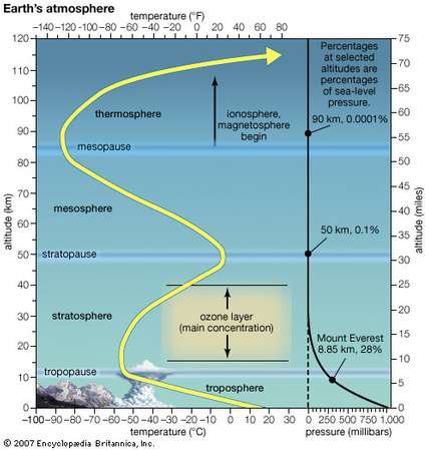
\includegraphics[height=0.22\textheight]{../figs/atmospheric-layers.png}\qquad
			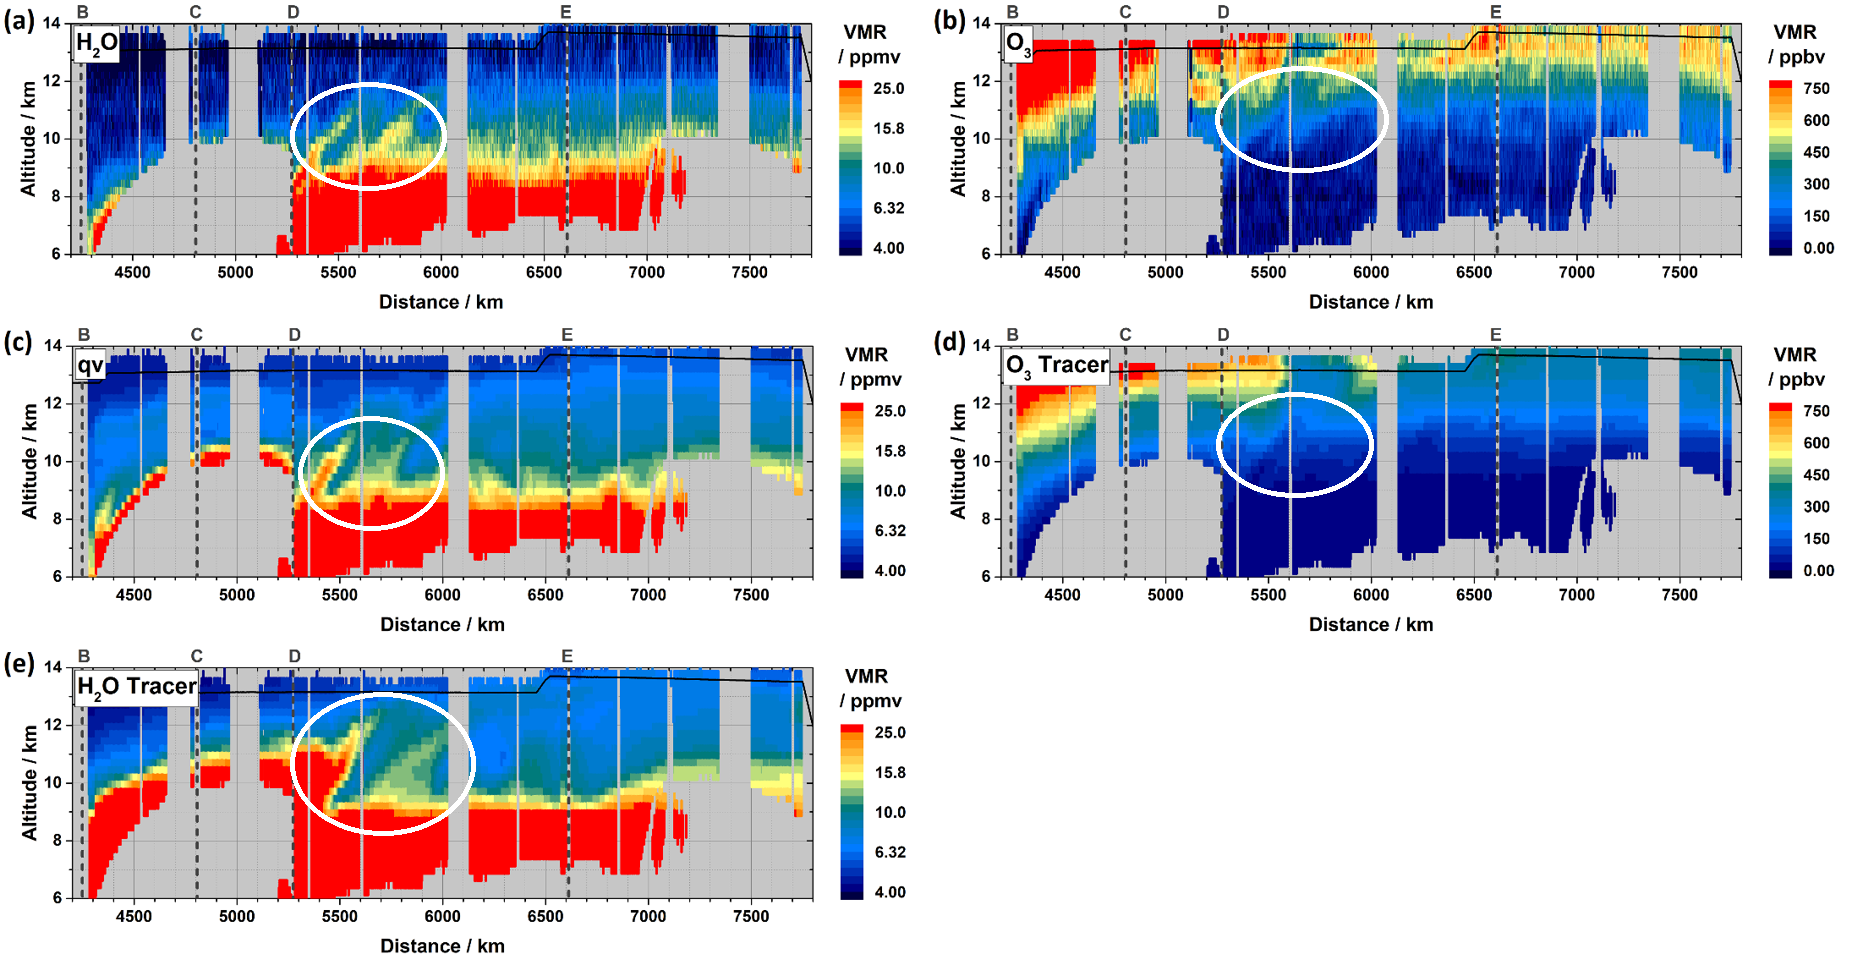
\includegraphics[height=0.22\textheight]{../figs/uplift}%
		}		
		\caption*{Left: The layers of the atmosphere, Right: Exemplary images of wave-like structures}
	\end{figure}

	{\bfseries Background information}\\
	With the help of airplanes, measured values from the Polar Vortex (PV) can be recorded. The value can be used to determine the layer of atmosphere in which the aircraft is currently located. The tropopause has a PV value of 2. This value can be used to determine the course of the tropopause.\\
	Measurements show that strong peaks and wave-like phenomena, as marked in the picture above, occur in this layer. It is not yet clear why they occur and what happens to them afterwards and how they influence our weather and temperature. \\
	
	{\bfseries Challenge}\\
	A detection tool is to be written which detects these wave-like locations in the simulation data and subsequently tracks them. 

\end{document}
% ----------------------------------------------------------%


